\documentclass[seminar]{fer}

\usepackage[authoryear]{natbib}
\usepackage{gensymb}
\title{Detekcija pješaka u urbanim okruženjima korišenjem značajki temeljenih na teksturi i boji}
\author{Iva Miholić, Gustav Matula, Kristijan Franković, Tomislav Kiš}
\makeindex

\begin{document}
\maketitle
\tableofcontents

\chapter{Detekcija pješaka u urbanim okruženjima}
\section{Opis projektnog zadatka}
Detekcija pješaka u urbanim okruženjima problem je povezan sa automobilskom industrijom, sigurnošću u prometu, sigurnosnim nadziranjem i robotikom. Rješava se kao detekcija objekta u okviru područja računalnog vida. Ovaj projektni zadatak obuhvaća izgradnju detektora pješaka na fotografijama iz urbanih okruženja korištenjem značajki temeljenih na bridovima,  teksturi i boji.

\section{Pregled i opis postojećih rješenja}

Pregled najznačajnijih rješenja ovog problema dan je u \cite{BenensonOHS14}. Trenutačno postoje dva glavna pristupa tom problemu. Prva klasa metoda obuhvaća detektore za pojedine dijelove tijela koji se zatim kombiniraju u detektor čvojeka - pješaka dok druga klasa prihvaća problemu statističkom analizom kombinirajući mnogobrojne značajke unutar detekcijskog prozora u klasifikator. 


Prvi značajniji napredak u detekciji pješaka bila je primjena \emph{VJ} detektora objekata \cite{VJ} na ovaj problem. Detektori temeljeni na histogramu usmjerenih gradijenata \engl{Histogram of Oriented Gradients, HOG} \cite{HOG}  uz linearni ili nelinearni skup potpornih vektora, postigli su značajne rezultate. No, primjena samo HOG značajki vodi do broja pogrešno pozitivno klasificiranih primjera čime se može stati na kraj uvodeći u sustav značajke temeljene na svojstvima boje, tekstura i oblika. 

Više o HOG pristupu bit će riječi u sljedećim poglavljima jer ćemo ga koristiti kao kostur našeg prostora značajki.

Od ostalih rezultata, potrebno je izdvojiti postupke temeljene na modelu rastavljivih dijelova  \engl{Deformable Part Models, DPM} u kojem se detekcija dijelova tijela sažima u detekciju cijelog pješaka te nelinearne postupke učenja temeljenih na neuronskim mrežama i stabalima odluke \cite{BenensonOHS14}. Takvi složeniji postupci uspoređeni su sa linearnim SVM-om uz HOG i druge značajke nisu dali značajno bolji rezultat upućujući na korektnost naše odluke o arhitekturi detektora.

Pristup na koji ćemo se fokusirati koristi metodu skalabilnog kliznog prozora. Unutar prozora na fotografiji određuju se značajke te se skup piksela unutar prozora binarno klasificira kao fotografija pješaka. Prozor zatim "putuje" po fotografiji testirajući druge skupove piksela. Slika se onda može dodatno skalirati (efektivno skalirajući prozor) nakon čega se ponavlja isti postupak. Primjer klasificirane fotografije ovakvim postupkom vidljiv je na slici \ref{primjer_klasifikacije}. Problem takvog pristupa je ignoriranje konteksta oko okvira koji se promatra što se uspješno rješava uvođenjem novih značajki, odnosno novih informacija o prozoru u sustav.

\begin{figure}
\center
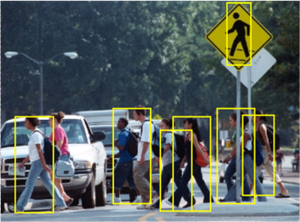
\includegraphics[scale=0.7]{img/crossing.png}
\caption{Fotografija koja je klasificirana detektorom pješaka metodom kliznog prozora. Žuti okviri prikazuju okvire onih prozora koji su klasificirani kao prikaz pješaka.}
\label{primjer_klasifikacije}
\end{figure}

Do sada su najviše korištene značajke temeljene na informaciji o bridovima, boji, teksturi loklalnim oblicima te svojstvima gradijenta i kovarijance. Dodavanje novih značajki pokazao se kao vrlo uspješan način poboljšanja rada detektora pješaka, no proširenje prostora značajki može biti problematično za klasične algoritme učenja što se rješava redukcijom prostora značajki metodom Fisherove diskriminantne analize,  analizom glavnih komponenti (\engl{Principal Component Analysis, PCA}, ili postupkom parcijalnih najmanjih kvadrata \engl{Partial Least Squares, PLS} \cite{Schwartz}. 

\section{Konceptualno rješenje zadatka}
\subsection{Pregled značajki temeljenih na teksturi i boji}

Promatrajući pješake na fotografijama, možemo uočiti karakteristike koje ih razlikuju od, na primjer, pozadine: vertikalni bridovi uz rub siluete, često uniformna boja odjeće, razlika u teksturi iste naspram teksturi pozadine, boja kože u području glave, ruku i nogu...  Motivacija za komplementiranjem značajki boje i teksture značajkama vezanim uz bridove (HOG deskriptori) tako se prirodno nameće kao bolji opis sustava. 

Značajke temeljene na teksturi i boji obično se koriste kao nadopuna značajkama fokusiranim na bridove, za koju ćemo koristiti popularnu HOG
metodu Dalal i Triggsa \cite{HOG}. Njihova se metoda pokazala dobrom na više baza podataka, ali promatranjem isključivo gradijenata potencijalno odbacujemo
korisne izvore informacija, što vodi lažnoj pozitivnoj klasifikaciji. Primjerice tekstura nam dosta pomaže kod prepoznavanja odjeće, ali i pozadine, a boja kod prepoznavanja boje kože.

\subsubsection{Histogram usmjerenih gradijenata ili HOG značajke}
%TODO

\subsubsection{Značajke temeljene na teksturi}
Vjerojatno najpoznatija metoda ekstrakcije značajki koje opisuju teksturu potječe iz Haralickovog rada \cite{Haralick} još iz 1979. Za opis teksture koristi takozvanu \emph{co-occurrence} matricu, iz koje se zatim računaju same značajke, kao što su npr. korelacija, srednje vrijednosti i razne mjere entropije.

Osnovna ideja iza matrice jest određivanje vjerojatnosti susjedstva svih parova intenziteta boje. Tako primjerice horizontalna matrica $H$ kao element
$h_{i,j}$ sadrži vjerojatnost da je nasumični par horizontalno susjednih piksela ima intenzitete redom $i$ i $j$. Matrica se tipično računa za horizontalni, vertikalni, te oba dijagonalna smjera (smjerovi $0\degree$, $45\degree$, $90\degree$, $135\degree$) . Još jedan parametar koji se može koristiti jest udaljenost $d$, pa tako matrica $V^{(d)}$ uzima u obzir 
parove koji su vertikalno susjedni na udaljenosti $d$.

Svaka tako dobivena matrica promatra se kao matrica zajedničke distribucije vjerojatnosti $p(i, j)$, te iz nje računamo značajke. Tipični primjeri značajki koje Haralick navodi u svome radu su primjerice:

\begin{itemize}
  \item
  varijanca: $$\sum_{i}\sum_{j}(i - \mu)^2p(i, j)$$
  \item
  korelacija: $$\frac{\sum_{i}\sum_{j}(ij)p(i,j) - \mu_{x}\mu_{y}}{\sigma_{x}\sigma_{y}}$$
  \item
  entropija: $$-\sum_{i}\sum_{j}p(i, j)\log(p(i, j))$$
\end{itemize}


\subsubsection{Značajke temeljene na boji}

U \cite{Schwartz} se za iskorištavanje informacije sadržane u boji koristi jednostavno proširenje HOG histograma. Tijekom izgrade HOG histograma, promatramo koji boji pripada gradijent s najvećom normom te se formira trostupčani histogram frekvencija svake od tri boje za trenutni prozor detekcije. Tako uz histogram gradijenata promatramo i histogram boja.

\subsection{Redukcija dimenzije}

Dovođenje mnogo značajki u sustav, odnosno visoka dimenzionalnost vektora značajki, može predstavljati problem za klasične tehnike učenje poput SVM-a, posebice uz često mali skup primjera za učenje.

Pretpostavimo (slično kao u \cite{Schwartz}) da je detekcijski prozor podijeljen na preklapajuće blokove u iz kojih se zatim ekstrahiraju opisane značajke. Vektori značajki za sve blokove istog prozora konkateniraju se u vektor značajki prozora. Velika dimenzija takvog prostora značajki koju dobivamo promatrajući, uz gradijente, teksturu i boju, predstavlja problem za klasične metode strojnog učenja. No, zbog podijele prozora detekcije u blokove, značajke se ekstrahiraju iz susjednih blokova, što neizbježno vodi do sličnih značajki u bliskim blokovima te samim time i do kolinearnosti. Tako ima smisla iskoristiti nekakvu tehniku redukcije dimenzije, kao što su
PCA (\emph{Principal Component Analysis}) ili FDA (\emph{Fisher Discriminant Analysis}). \cite{Schwartz} koristi PLS (\emph{Partial Least Squares}), inače 
regresijsku metodu, praktičnu i za redukciju dimenzije skupa značajki zbog njene brzine i primjenjivosti na ovaj specifičan model.

Nakon redukcije dimenzije za treniranje klasifikatora možemo koristiti metode učenja kao što je SVM (\emph{Support Vector Machine}) koje bi na prostoru s 
previše dimenzija bile neupotrebljive.

\subsection{Plan arhitekture sustava računalnog vida}

Sustav će se kao i obično sastojati od dvije osnovne komponente: treniranja i testiranja te primjene.

\subsubsection{Treniranje klasifikatora}

\begin{figure}[h!]
\center
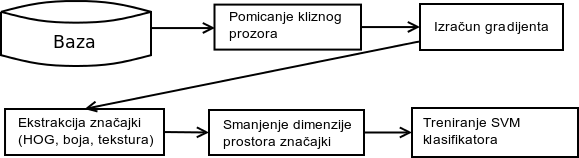
\includegraphics[scale=0.7]{img/treniranje.png}
\caption{Dijagram treniranja SVM klasifikatora}
\label{treniranje}
\end{figure}

Treniranje se sastoji od nekoliko koraka koji su okvirno prikazani na slici \ref{treniranje}.
Za svaku sliku iz baze računaju se gradijenti (horizontalni i vertikalni smjer). Zatim po slici pomičemo
klizni prozor, dijelimo ga na preklapajuće blokove i za svaki blok računamo histogram gradijenata i histogram boja. Prozor potom ponovno dijelimo
na blokove (ne nužno istih dimenzija kao u prethodnom koraku), te računamo \emph{co-occurrence} matrice za sva četiri smijera i udaljenost $d = 1$ matricu, iz kojih dobivamo značajke koje opisuju
teksturu. U sljedećem koraku reduciramo dimenziju prostora značajki. Konačno, na tako pojednostavljenim primjerima treniramo SVM. U tijeku postupka parametri metode redukcije i SVM-a dobivaju se metodom 10-koračne križne validacije (\emph{$10$-fold-cross-validation}.

\subsubsection{Testiranje klasifikatora}

Novotreniranom klasifikatoru ćemo zatim testirati sposobnost generalizacije i pretreniranost. 
%TODO 

\subsubsection{Primjena klasifikatora}

Slično kao kod treniranja promatramo klizni prozor i za njega računamo značajke, kojima zatim reduciramo dimenziju te ih dajemo kao ulazne podatke klasifikatoru. Ukoliko klasifikator procijeni da se radi o pješaku, dojavljujemo poziciju trenutnog kliznog prozora.

\chapter{Postupak rješavanja zadatka} %TODO
\section{Ekstrakcija značajki}
\section{Treniranje prve faze klasifikatora}
\section{Treniranje druge faze klasifikatora}


\chapter{Ispitivanje rješenja}
\section{Ispitna baza}

Za treniranje i verifikaciju rješenja koristit ćemo skup podataka INRIA \cite{DT05}. To je skup fotografija urbanog okruženja u boji i pripadnih anotacija. Za svaku fotografiju zabilježen je skup graničnih prozora \engl{bounding window} unutar kojih se nalaze prikazi uspravnih osoba.

INRIA se do sada često koristio za trening detektora zbog raznolikosti pozadinskih okruženja osoba na slikama i točnosti anotacija \cite{BenensonOHS14}. Za razliku od ostalih javno dostupnih baza podataka za detekciju pješaka, ove fotografije nisu dobivene iz videa te su relativno visoke kvalitete i fotografirane su iz različitih točaka gledišta. U drugim bazama podataka, pješaci su većinom konecentrirani u centralnoj horizontali fotografije jer je ista dobivena iz vozačeve perspektive.
\begin{figure}[h!]
\centering
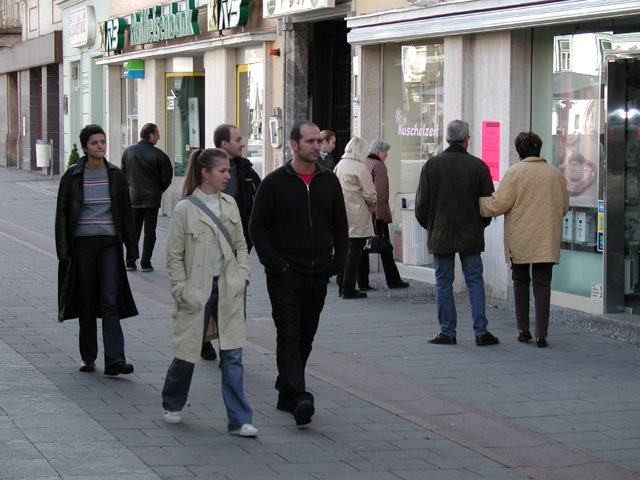
\includegraphics[scale=1.7]{img/person_139.png}
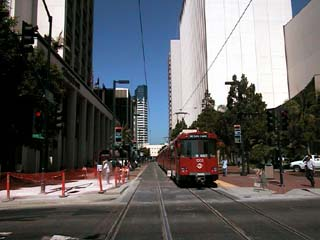
\includegraphics[scale=0.5]{img/neg.png}
\caption{Primjeri fotografija iz baze podataka INRIA.}
\label{inria1}
\end{figure}

Baza slika INRIA sadrži slike iz nekoliko različitih izvora:
\begin{itemize}
\item \emph{Graz 01} skup podataka sa pridodanim bilješkama
\item slike iz osobne kolekcije samog autora koje su zbog svoje veličine u originalu izrezane tako da prikazuju samo osobu
\item slike sa servisa Google Images
\end{itemize}.

Sama se baza sastoji od podskupa podataka za trening i podskupa za evaluaciju. U podskupu za trening označena su $1208$ pješaka u $614$ od $1832$ fotografije. U podskupu za testiranje označeno je $566$ pješaka u $453$ od $741$ fotografije \cite{Dollar:2012:PDE:2197081.2197275}.  Primjeri fotografija sa i bez pješaka dani su na slici \ref{inria1}. Primjer anotacije za lijevu fotografiju sa slike \ref{inria1} dan je na slici \ref{inria2}.

\begin{figure}[h!]
\centering
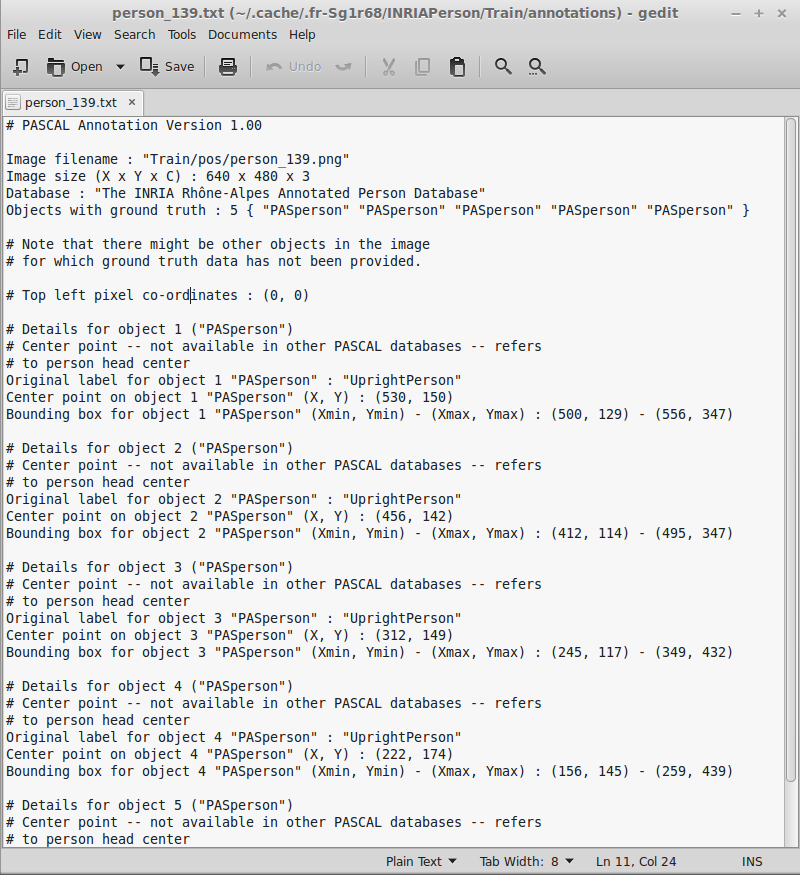
\includegraphics[scale=0.3]{img/annot_139.png}
\caption{Primjer anotacije pozitivno klasificiranih kliznih prozora za lijevu fotografiju na slici \ref{inria1}.}
\label{inria2}
\end{figure}

\section{Rezultati učenja i ispitivanja}
%TODO

\section{Analiza rezultata}
%TODO

\bibliographystyle{plain}
\bibliography{bibliografija}
\end{document}
